\documentclass[12pt,a4paper]{article}

% ── Encodage et langue ─────────────────────────────────────────────────────
\usepackage[utf8]{inputenc}
\usepackage[T1]{fontenc}


% ── Mise en page ───────────────────────────────────────────────────────────
\usepackage[top=2.5cm,bottom=2.5cm,left=3cm,right=2.5cm,headheight=15pt]{geometry}
\usepackage{setspace}
\onehalfspacing

% ── Graphiques et figures ──────────────────────────────────────────────────
\usepackage{pgfplots}
\pgfplotsset{compat=1.18}
\usepackage{pgfplotstable}
\usepackage{tikz}
\usetikzlibrary{patterns,decorations.pathreplacing}

% ── Tableaux ───────────────────────────────────────────────────────────────
\usepackage{booktabs}
\usepackage{multirow}
\usepackage{array}
\usepackage{tabularx}
\usepackage{longtable}
\usepackage{colortbl}

% ── Couleurs ───────────────────────────────────────────────────────────────
\usepackage{xcolor}
\definecolor{congoblue}{RGB}{0,68,130}
\definecolor{gabongreen}{RGB}{0,158,96}
\definecolor{tchadyellow}{RGB}{200,150,0}
\definecolor{lightgray}{RGB}{240,240,240}
\definecolor{darkgray}{RGB}{80,80,80}

% ── Liens et PDF ───────────────────────────────────────────────────────────
\usepackage[hidelinks,
            pdfauthor={Georges Miguel Moukoko Ekambi},
            pdftitle={Analyse de la Balance des Paiements : Congo, Gabon, Tchad -- 2021},
            pdfsubject={Économie internationale -- CEMAC}]{hyperref}

% ── Bibliographie ──────────────────────────────────────────────────────────
\usepackage[backend=biber,style=apa,sorting=nyt]{biblatex}
\addbibresource{references.bib}

% ── Mathématiques ──────────────────────────────────────────────────────────
\usepackage{amsmath,amssymb}

% ── Entêtes et pieds de page ───────────────────────────────────────────────
\usepackage{fancyhdr}
\pagestyle{fancy}
\fancyhf{}
\fancyhead[L]{\small\textit{Analyse BDP -- Congo, Gabon, Tchad (2021)}}
\fancyhead[R]{\small\textit{G.M. Moukoko Ekambi}}
\fancyfoot[C]{\thepage}
\renewcommand{\headrulewidth}{0.4pt}

% ── Sections personnalisées ────────────────────────────────────────────────
\usepackage{titlesec}
\titleformat{\section}{\large\bfseries\color{congoblue}}{{\thesection}}{1em}{}
\titleformat{\subsection}{\normalsize\bfseries\color{darkgray}}{{\thesubsection}}{1em}{}

% ── Captions ───────────────────────────────────────────────────────────────
\usepackage{caption}
\captionsetup{font=small,labelfont=bf,labelsep=period}

% ── Abstract personnalisé ──────────────────────────────────────────────────
\usepackage{abstract}
\renewcommand{\abstractnamefont}{\normalfont\bfseries}

% ── Numérotation des figures et tableaux ───────────────────────────────────
\usepackage{chngcntr}

%% ══════════════════════════════════════════════════════════════════════════
%%  DÉBUT DU DOCUMENT
%% ══════════════════════════════════════════════════════════════════════════
\begin{document}

% ─── Page de titre ──────────────────────────────────────────────────────────
\begin{titlepage}
  \centering
  {\small UNIVERSITÉ DE DOUALA\\
  ÉCOLE NATIONALE SUPÉRIEURE POLYTECHNIQUE DE DOUALA (ENSPD)\\
  Master 2 -- Données, Sciences et Intelligence Artificielle (SDIA)}

  \vspace{1cm}
  \rule{\linewidth}{0.5pt}
  \vspace{0.5cm}

  {\LARGE\bfseries\color{congoblue}
    Analyse comparative de la Balance des Paiements\\[0.4cm]
    République du Congo, République du Gabon\\
    et République du Tchad\\[0.3cm]
    -- Exercice 2021 --}

  \vspace{0.5cm}
  \rule{\linewidth}{0.5pt}

  \vspace{1.2cm}
  {\large\itshape Rapport scientifique}

  \vfill

  \begin{tabular}{ll}
    \textbf{Auteur :}        & Georges Miguel Moukoko Ekambi \\[4pt]
    \textbf{Superviseurs académique :}  & Prof. Dr. habil. P. Njionou Sadjang \\
                             & Dr. Kenmoe \\[4pt]
    \textbf{Source officielle :} & BEAC -- Direction Nationale, exercice 2021 \\[4pt]
    \textbf{Norme :}         & BPM6 (FMI, 2009) \\[4pt]
    \textbf{Date :}          & \today
  \end{tabular}

  \vspace{1cm}
\end{titlepage}

% ─── Résumé ─────────────────────────────────────────────────────────────────
\begin{abstract}
Ce rapport analyse et compare la balance des paiements (BDP) de la République du Congo,
de la République Gabonaise et de la République du Tchad pour l'exercice 2021, à partir des
données statistiques officielles publiées par la Banque des États de l'Afrique Centrale
(BEAC) conformément à la norme BPM6 du Fonds Monétaire International (FMI, 2009). L'étude
examine les principaux soldes -- compte courant, compte de capital, compte financier -- et
leurs implications macroéconomiques, les termes d'échange extérieurs, et la soutenabilité
des positions extérieures de chaque pays. Les résultats montrent que les trois économies,
bien qu'excédentaires en courant en 2021 grâce au rebond des prix pétroliers, présentent des
vulnérabilités structurelles communes caractéristiques du syndrome hollandais
\parencite{cordenneary1982} : déficits profonds des services et du revenu primaire, forte
dépendance aux investisseurs étrangers, et taux de rétention des revenus d'exportation
inférieur à 65\,\%. Ces résultats appellent des politiques de diversification économique
urgentes dans les trois pays membres de la CEMAC.
\end{abstract}

\newpage
\tableofcontents
\newpage

%% ══════════════════════════════════════════════════════════════════════════
\section{Introduction}
%% ══════════════════════════════════════════════════════════════════════════

La balance des paiements constitue un instrument statistique fondamental de la comptabilité
nationale internationale. Elle retrace l'ensemble des transactions économiques et financières
réalisées entre les résidents d'un pays et le reste du monde au cours d'une période donnée,
généralement une année \parencite{imf2009bpm6}. Son analyse permet non seulement de mesurer
les flux d'échanges extérieurs, mais aussi d'identifier les déséquilibres structurels et
d'orienter les politiques économiques \parencite{krugmanobstfeld2018}.

Dans le contexte de la Communauté Économique et Monétaire de l'Afrique Centrale (CEMAC),
la balance des paiements revêt une importance particulière. Les économies membres sont
fortement dépendantes des exportations de ressources naturelles, dont le pétrole constitue
le principal moteur. Cette dépendance, bien documentée dans la littérature sous le concept
de « malédiction des ressources naturelles » \parencite{sachswarner1995}, crée une
vulnérabilité structurelle aux chocs extérieurs et génère des déséquilibres profonds dans
les différents comptes de la balance des paiements.

Le présent rapport porte sur trois pays membres de la CEMAC -- la République du Congo, la
République Gabonaise et la République du Tchad -- pour l'exercice 2021. Cette année est
particulièrement intéressante à analyser car elle correspond à une reprise post-Covid des
cours pétroliers, créant des conditions de termes d'échange favorables qui peuvent masquer
des fragilités structurelles profondes.

Les données utilisées proviennent exclusivement des fichiers officiels de la BEAC,
accessibles sur le portail \textit{Économie et Statistiques} à l'adresse
\url{https://www.beac.int/economie-stats/statistiques-de-balance-paiements/}. Ces données
sont établies conformément à la sixième édition du Manuel de la Balance des Paiements et de
la Position Extérieure Globale (BPM6) du FMI \parencite{imf2009bpm6}, qui constitue la
norme internationale de référence depuis 2009.

Ce rapport s'articule autour de trois parties : une revue de la littérature théorique et
empirique sur la balance des paiements des économies pétrolières, une présentation de la
méthodologie d'analyse, et enfin une présentation détaillée des résultats avec leur
interprétation économique comparée.

%% ══════════════════════════════════════════════════════════════════════════
\section{Revue de la littérature}
%% ══════════════════════════════════════════════════════════════════════════

\subsection{Le cadre conceptuel de la balance des paiements}

La balance des paiements est définie par le FMI comme « un état statistique qui résume,
pour une période donnée, les transactions économiques d'une économie avec le reste du monde »
\parencite[p.~9]{imf2009bpm6}. La sixième édition du manuel BPM6, publiée en 2009, organise
ces transactions en trois comptes principaux : le compte des transactions courantes, le
compte de capital et le compte financier, auxquels s'ajoute un poste d'erreurs et d'omissions
servant de variable d'ajustement statistique.

Le compte courant enregistre les biens, les services, les revenus primaires et les revenus
secondaires. Le compte de capital retrace les transferts en capital et les acquisitions ou
cessions d'actifs non financiers non produits. Le compte financier, quant à lui, récence
les investissements directs, les investissements de portefeuille, les dérivés financiers,
les autres investissements et les avoirs de réserve \parencite{imf2009bpm6}.

Une identité comptable fondamentale structure l'ensemble du système :

\begin{equation}
  B_{courant} + B_{capital} + B_{financier} + E\&O = 0
  \label{eq:identite_bdp}
\end{equation}

où $B_{courant}$, $B_{capital}$ et $B_{financier}$ désignent respectivement les soldes des
trois comptes, et $E\&O$ le poste d'erreurs et d'omissions. Cette identité implique que tout
déficit du compte courant doit nécessairement être financé par un excédent du compte
financier, c'est-à-dire par des entrées nettes de capitaux \parencite{krugmanobstfeld2018}.

\subsection{La théorie des termes d'échange}

Les termes d'échange mesurent le rapport entre l'indice des prix à l'exportation et l'indice
des prix à l'importation d'un pays. Une amélioration des termes d'échange signifie que le
pays reçoit des prix plus élevés pour ses exportations relativement à ses importations,
ce qui améliore mécaniquement le solde commercial \parencite{prebischsinger1950}. Pour les
économies exportatrices de matières premières, les termes d'échange sont déterminés de
manière exogène par les marchés internationaux, créant une volatilité macroéconomique
structurelle.

\textcite{prebischsinger1950} ont montré, dans leur thèse sur la détérioration séculaire des
termes d'échange, que les pays exportateurs de produits primaires font face à une tendance
de long terme à la détérioration de leur position commerciale par rapport aux pays
industrialisés, en raison de l'inélasticité-revenu des matières premières. Bien que cette
thèse ait été partiellement révisée depuis, elle reste pertinente pour comprendre la
vulnérabilité structurelle des économies pétrolières.

\subsection{Le syndrome hollandais dans les économies pétrolières}

Le concept central permettant d'analyser les déséquilibres de la balance des paiements dans
les économies pétrolières est celui du syndrome hollandais (\textit{Dutch Disease}), théorisé
par \textcite{cordenneary1982} dans leur modèle canonique. Ce modèle distingue trois secteurs
dans une petite économie ouverte : un secteur en boom (les ressources naturelles), un secteur
en retard (l'industrie manufacturière), et un secteur de non-échangeables (les services).

Selon \textcite{cordenneary1982}, un boom d'exportation de ressources naturelles produit deux
effets majeurs. Premièrement, un \textit{effet de déplacement des ressources} : les facteurs
de production migrent vers le secteur en boom, appauvrissant les autres secteurs. Deuxièmement,
un \textit{effet de dépense} : l'afflux de revenus pétroliers augmente la demande de biens
non-échangeables (services), entraînant une appréciation réelle du taux de change qui pénalise
la compétitivité des exportations non-pétrolières. \textcite{corden1984} a par la suite
consolidé et étendu cette analyse.

\textcite{wijnbergen1984} a approfondi le modèle initial en y intégrant le rôle des
anticipations et des dynamiques intertemporelles, montrant comment les booms pétroliers
affectent l'épargne nationale, la balance extérieure et l'accumulation du capital. Dans la
balance des paiements, ces effets se manifestent par des déficits croissants du compte des
services -- les entreprises étrangères captant la valeur ajoutée autour de l'extraction --
et du revenu primaire -- les profits et dividendes partant à l'étranger.

\subsection{La malédiction des ressources naturelles dans la CEMAC}

\textcite{sachswarner1995}, dans leur étude économétrique pionnière publiée comme
\textit{NBER Working Paper}, ont montré empiriquement que la dépendance aux exportations
de ressources naturelles est corrélée négativement à la croissance économique sur données
de panel, après contrôle des autres caractéristiques structurelles des économies. Leurs
résultats, confirmés dans \textcite{sachswarner2001}, suggèrent que les pays abondants en
ressources naturelles tendent à croître moins vite que les pays pauvres en ressources.

Dans le contexte spécifique de la CEMAC, \textcite{beac2023} documentent une dépendance
persistante des recettes fiscales aux revenus pétroliers, caractéristique qui détériore la
prévisibilité budgétaire des secteurs sociaux et réduit l'efficacité des dépenses publiques
à long terme. \textcite{imfcemac2021} soulignent que les économies de la sous-région sont
exposées à un risque d'insoutenabilité de la position extérieure en cas de baisse prolongée
des cours pétroliers, eu égard à la structure de leur balance des paiements.

Pour le Tchad en particulier, \textcite{peggetchad2005} analyse la loi de gestion des
revenus pétroliers, qui visait précisément à contrôler les risques de syndrome hollandais
en imposant une affectation réglementée des recettes pétrolières et en constituant une
épargne systématique. Cette loi illustre la conscience des décideurs de la fragilité
structurelle de l'économie tchadienne face aux chocs pétroliers.

\subsection{Synthèse de la littérature}

La revue de la littérature met en évidence quatre enseignements qui cadrent notre analyse
empirique. Premièrement, les économies pétrolières génèrent structurellement des excédents
commerciaux masquant des déficits profonds des services et du revenu primaire. Deuxièmement,
les termes d'échange des pays exportateurs de pétrole sont déterminés de manière exogène
et volatile. Troisièmement, la malédiction des ressources naturelles se manifeste, dans la
balance des paiements, par une faible rétention des revenus d'exportation. Quatrièmement,
la politique économique doit viser la diversification des exportations pour réduire cette
vulnérabilité structurelle.

%% ══════════════════════════════════════════════════════════════════════════
\section{Méthodologie}
%% ══════════════════════════════════════════════════════════════════════════

\subsection{Sources des données}

Les données utilisées dans ce rapport proviennent de deux sources principales. La source
primaire est constituée des fichiers officiels de la BEAC, téléchargés sur le portail
\textit{Économie et Statistiques -- Statistiques de la Balance des Paiements} :

\begin{itemize}
  \item \textbf{Congo :} \textit{Balance des Paiements type provisoire de l'exercice 2021,
        arrêtée au 31/12/2021} (fichiers BDP\_CONGO\_2021 et Balance-des-Paiements-Analytique-2021-COG)
  \item \textbf{Gabon :} \textit{Balance des Paiements type provisoire de l'exercice 2021,
        arrêtée au 31/12/2021} (fichiers BDP\_GABON\_2021 et Balance-des-Paiements-analytique-2021-GABON)
  \item \textbf{Tchad :} \textit{Balance des Paiements type provisoire de l'exercice 2021,
        arrêtée au 31/12/2021} (fichier BDP\_TCHAD\_2021)
\end{itemize}

Il convient de noter que la \textbf{dernière balance des paiements disponible en ligne}
pour les trois pays, au moment de la rédaction de ce rapport, est celle de \textbf{l'exercice
2023} (accessible sur \url{https://www.beac.int/economie-stats/statistiques-de-balance-paiements/}).
Notre étude porte néanmoins sur l'exercice 2021, année pour laquelle les données des trois
pays sont complètes et homogènes.

Les données de PIB utilisées pour le calcul des ratios proviennent des \textit{World Economic
Outlook} du FMI (édition 2022), converties en millions de FCFA au taux de parité applicable.
Toutes les données monétaires sont exprimées en \textbf{millions de FCFA}.

\subsection{Norme de compilation}

Les données sont compilées conformément à la sixième édition du Manuel de la Balance des
Paiements et de la Position Extérieure Globale (BPM6) du FMI \parencite{imf2009bpm6},
publié en 2009. Cette norme, adoptée par la BEAC pour l'ensemble des pays membres de la
CEMAC, garantit la comparabilité internationale des données et la cohérence des concepts
utilisés. Trois facteurs ont guidé la révision du BPM5 vers le BPM6 : la mondialisation,
l'accent accru sur les bilans dans la position extérieure globale, et l'innovation financière
\parencite{ecbbpm6}.

\subsection{Indicateurs analysés}

L'analyse porte sur les soldes et ratios suivants :

\textbf{Soldes primaires de la BDP :}
\begin{align}
  S_{courant}  &= \text{Crédit}_{courant} - \text{Débit}_{courant} \label{eq:solde_courant}\\
  S_{capital}  &= \text{Crédit}_{capital} - \text{Débit}_{capital} \label{eq:solde_capital}\\
  S_{financier}&= \text{Actifs nets acquis} - \text{Passifs nets émis} \label{eq:solde_fin}
\end{align}

\textbf{Capacité ou besoin de financement :}
\begin{equation}
  CF = S_{courant} + S_{capital}
  \label{eq:cf}
\end{equation}

\textbf{Ratio solde courant / PIB :}
\begin{equation}
  r_{PIB} = \frac{S_{courant}}{PIB} \times 100
  \label{eq:ratio_pib}
\end{equation}

\textbf{Taux de couverture des biens (proxy des termes d'échange) :}
\begin{equation}
  TC = \frac{\text{Exportations de biens}}{\text{Importations de biens}}
  \label{eq:tc}
\end{equation}

\textbf{Taux d'absorption des services :}
\begin{equation}
  TAS = \frac{|\text{Déficit des services}|}{\text{Exportations de biens}} \times 100
  \label{eq:tas}
\end{equation}

\textbf{Taux de fuite du revenu primaire :}
\begin{equation}
  TFR = \frac{|\text{Déficit du revenu primaire}|}{\text{Exportations de biens}} \times 100
  \label{eq:tfr}
\end{equation}

\textbf{Taux de rétention des exportations (TRE) :}
\begin{equation}
  TRE = 100 - TAS - TFR
  \label{eq:tre}
\end{equation}

\subsection{Limites méthodologiques}

Trois limites doivent être signalées. Premièrement, les données BEAC sont qualifiées de
\textit{provisoires}, ce qui signifie qu'elles sont susceptibles de révision ultérieure.
Deuxièmement, le poste erreurs et omissions du Gabon (+310 772 M FCFA) représente près de
85\,\% de l'excédent courant, ce qui traduit des lacunes statistiques importantes dans les
données gabonaises de 2021. Troisièmement, l'absence d'indices de prix désagrégés pour les
exportations et importations empêche le calcul direct des termes d'échange au sens de la
définition standard ; le taux de couverture des biens (équation \ref{eq:tc}) est utilisé
comme approximation.

%% ══════════════════════════════════════════════════════════════════════════
\section{Résultats et Interprétations}
%% ══════════════════════════════════════════════════════════════════════════

\subsection{Les principaux soldes de la balance des paiements}

Le tableau \ref{tab:soldes_principaux} présente les soldes des trois comptes principaux
pour les trois pays en 2021, exprimés en millions de FCFA.

\begin{table}[h!]
  \centering
  \caption{Principaux soldes de la BDP -- Congo, Gabon, Tchad (2021, M FCFA)}
  \label{tab:soldes_principaux}
  \small
  \begin{tabular}{lrrr}
    \toprule
    \textbf{Poste} & \textbf{Congo} & \textbf{Gabon} & \textbf{Tchad} \\
    \midrule
    \rowcolor{lightgray}
    \textbf{Compte courant} & \textbf{+951\,523} & \textbf{+373\,630} & \textbf{+476\,748} \\
    \quad Biens et Services & +1\,810\,469 & +1\,045\,830 & +654\,335 \\
    \quad\quad Biens        & +2\,624\,146 & +2\,072\,410 & +1\,101\,693 \\
    \quad\quad Services     &   $-$813\,677 & $-$1\,026\,580 & $-$447\,358 \\
    \quad Revenu primaire   &   $-$915\,344 &   $-$639\,322 & $-$325\,471 \\
    \quad Revenu secondaire &    +56\,398 &    $-$32\,878 & +147\,884 \\
    \midrule
    \rowcolor{lightgray}
    \textbf{Compte de capital} & \textbf{+13\,772} & \textbf{+41} & \textbf{+143\,603} \\
    \midrule
    \rowcolor{lightgray}
    \textbf{Capacité de financement} & \textbf{+965\,295} & \textbf{+351\,664} & \textbf{+620\,351} \\
    \midrule
    \rowcolor{lightgray}
    \textbf{Compte financier (net)} & \textbf{$-$999\,773} & \textbf{$-$662\,436} & \textbf{$-$387\,202} \\
    \midrule
    Erreurs et omissions & +34\,478 & +310\,772 & $-$233\,149 \\
    \bottomrule
  \end{tabular}

  \smallskip
  \footnotesize\textit{Source : Fichiers BDP officiels BEAC, exercice 2021 (données provisoires).}
\end{table}

\begin{figure}[h!]
  \centering
  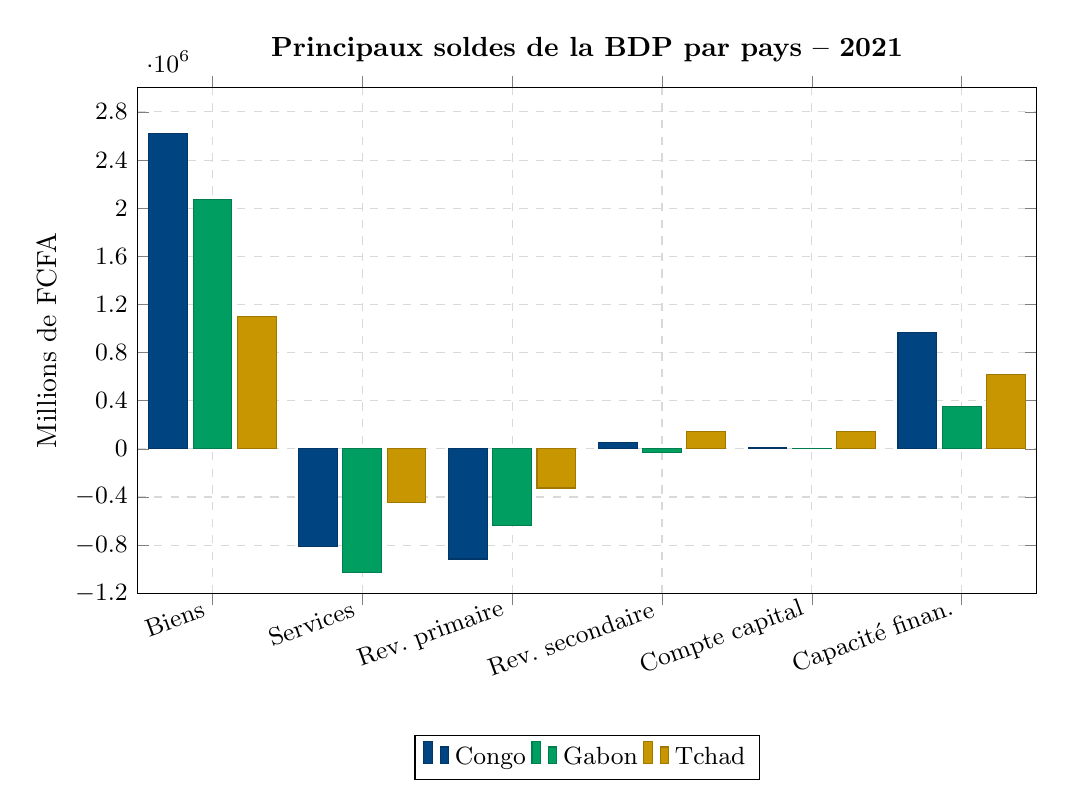
\begin{tikzpicture}
    \begin{axis}[
      ybar,
      width=13cm, height=8cm,
      bar width=14pt,
      xlabel={},
      ylabel={Millions de FCFA},
      xtick=data,
      xticklabels={Biens, Services, Rev.\ primaire, Rev.\ secondaire, Compte capital, Capacité finan.},
      xticklabel style={font=\small, rotate=20, anchor=east},
      ymin=-1200000, ymax=3000000,
      ytick={-1200000,-800000,-400000,0,400000,800000,1200000,1600000,2000000,2400000,2800000},
      yticklabel style={font=\small},
      legend style={at={(0.5,-0.28)}, anchor=north, legend columns=3, font=\small},
      legend cell align=left,
      title={\textbf{Principaux soldes de la BDP par pays -- 2021}},
      title style={font=\normalsize\bfseries},
      grid=major, grid style={dashed,gray!30},
      enlarge x limits=0.1,
    ]
    % Congo
    \addplot[fill=congoblue, draw=congoblue!80!black] coordinates {
      (1, 2624146) (2,-813677) (3,-915344) (4,56398) (5,13772) (6,965295)
    };
    % Gabon
    \addplot[fill=gabongreen, draw=gabongreen!80!black] coordinates {
      (1, 2072410) (2,-1026580) (3,-639322) (4,-32878) (5,41) (6,351664)
    };
    % Tchad
    \addplot[fill=tchadyellow, draw=tchadyellow!80!black] coordinates {
      (1, 1101693) (2,-447358) (3,-325471) (4,147884) (5,143603) (6,620351)
    };
    \legend{Congo, Gabon, Tchad}
    \end{axis}
  \end{tikzpicture}
  \caption{Principaux soldes de la balance des paiements -- Congo, Gabon, Tchad (2021)}
  \label{fig:soldes_principaux}
\end{figure}

\paragraph{Interprétation.}
Les trois pays affichent un excédent du compte courant en 2021, avec le Congo en tête
(+951\,523 M FCFA), suivi du Tchad (+476\,748 M FCFA) et du Gabon (+373\,630 M FCFA).
Cependant, comme le montre la figure \ref{fig:soldes_principaux}, cette apparence favorable
masque des déséquilibres profonds. Le solde des biens est largement excédentaire dans les
trois pays grâce aux exportations pétrolières, mais il est presqu'entièrement absorbé par
les déficits des services et du revenu primaire. Ce profil illustre le mécanisme du syndrome
hollandais décrit par \textcite{cordenneary1982} : la rente pétrolière génère un excédent
commercial mais enrichit les opérateurs étrangers via les services facturés et les profits
rapatriés, réduisant drastiquement la rétention nationale de la valeur créée.

\subsection{Implications des soldes : excédent ou déficit}

\subsubsection{Un excédent courant structurellement vulnérable}

Un excédent du compte courant signifie que le pays reçoit davantage de ressources de
l'extérieur qu'il n'en verse sur l'ensemble de ses transactions courantes. Cela induit
une \textit{capacité de financement} vis-à-vis du reste du monde : théoriquement, le pays
prête plus à l'étranger qu'il n'emprunte. En pratique, dans les trois cas, cette capacité
se matérialise par des sorties de capitaux via le compte financier, reflétant les bénéfices
réinvestis des compagnies pétrolières étrangères et les dépôts bancaires externes des
opérateurs du secteur extractif.

L'implication centrale est la \textbf{fragilité de cet excédent} : il repose entièrement
sur une ressource épuisable dont les prix sont déterminés exogènement. Ainsi, la baisse des
cours pétroliers observée à partir de 2022 a conduit le compte courant du Gabon à se
contracter de 1\,083 milliards à 452 milliards de FCFA entre 2022 et 2023
\parencite{beac2023rapport}.

\subsubsection{Le déficit des services : signal d'enclavement productif}

Le déficit persistant des services dans les trois économies révèle leur enclavement dans la
chaîne de valeur pétrolière. Le Congo verse 813\,677 M FCFA nets en services à l'étranger,
le Gabon 1\,026\,580 M FCFA, et le Tchad 447\,358 M FCFA. Ces sorties correspondent
principalement aux services d'assistance technique, de location d'équipements et de conseils
facturés par les multinationales pétrolières à leurs filiales locales. Comme le souligne
\textcite{cordenneary1982}, le secteur extractif fonctionnant comme une enclave ne génère
pas d'externalités technologiques vers le reste de l'économie, perpétuant la dépendance
aux prestataires étrangers.

\subsubsection{Le déficit du revenu primaire : la capture des profits}

Le déficit du revenu primaire est particulièrement révélateur. Le Congo transfère 915\,344
M FCFA aux investisseurs étrangers, le Gabon 639\,322 M FCFA et le Tchad 325\,471 M FCFA.
La composante dominante est systématiquement les bénéfices réinvestis des entreprises
d'investissement direct : 628\,308 M FCFA pour le Congo, 247\,995 M FCFA pour le Gabon.
Ces bénéfices, même lorsqu'ils sont physiquement réinvestis dans le pays hôte, sont
comptabilisés comme une sortie de revenu car ils appartiennent aux actionnaires non-résidents
\parencite{imf2009bpm6}. Ce mécanisme confirme l'analyse de \textcite{sachswarner1995} sur
l'impossibilité pour les pays riches en ressources de convertir leur richesse brute en
développement économique durable.

\subsection{Les termes d'échange vis-à-vis de l'extérieur}

\subsubsection{Mesure et résultats}

En l'absence d'indices de prix désagrégés dans les fichiers BEAC, les termes d'échange sont
approchés par le taux de couverture des biens (équation \ref{eq:tc}), qui exprime le montant
des exportations de biens pour chaque unité monétaire importée.

\begin{table}[h!]
  \centering
  \caption{Indicateurs t de rétention des exportations (2021)}
  \label{tab:termes_echange}
  \begin{tabular}{lrrr}
    \toprule
    \textbf{Indicateur} & \textbf{Congo} & \textbf{Gabon} & \textbf{Tchad} \\
    \midrule
    Exportations de biens (M FCFA)    & 4\,165\,400 & 3\,987\,576 & 2\,165\,570 \\
    Importations de biens (M FCFA)    & 1\,541\,254 & 1\,915\,166 & 1\,063\,877 \\
    \textbf{Taux de couverture (TC)}  & \textbf{2,70} & \textbf{2,08} & \textbf{2,04} \\
    \midrule
    Taux d'absorption services (\%)   & 19,5 & 25,7 & 20,7 \\
    Taux de fuite rev. primaire (\%)  & 22,0 & 16,0 & 15,0 \\
    \textbf{Taux de rétention (\%)}   & \textbf{58,5} & \textbf{58,3} & \textbf{64,3} \\
    \bottomrule
  \end{tabular}

  \smallskip
  \footnotesize\textit{Source : Calculs de l'auteur à partir des fichiers BEAC 2021.}
\end{table}

\begin{figure}[h!]
  \centering
  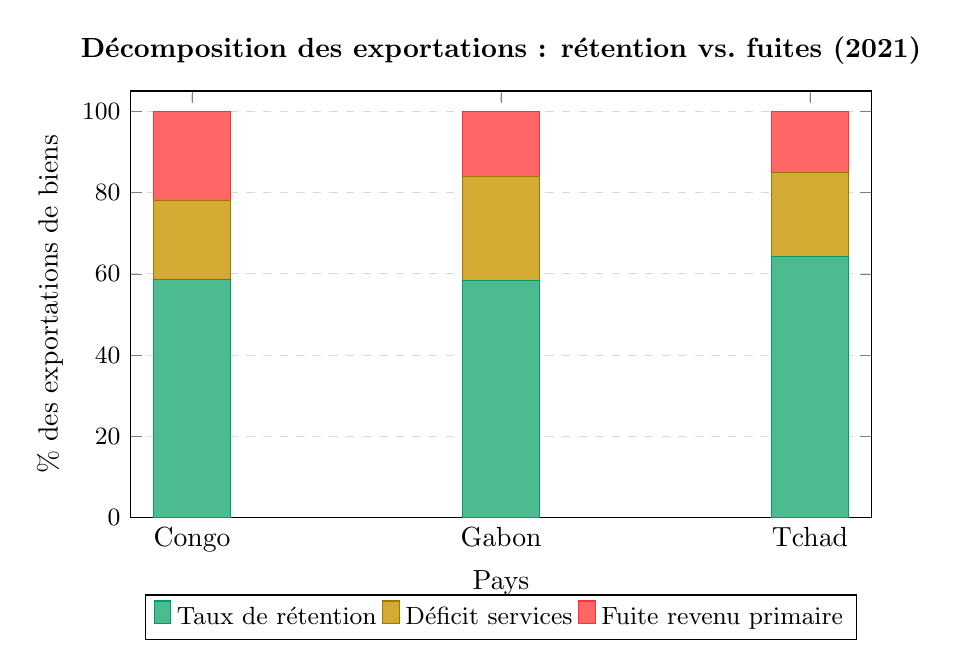
\begin{tikzpicture}
    \begin{axis}[
      ybar stacked,
      width=11cm, height=7cm,
      bar width=28pt,
      xlabel={Pays},
      ylabel={\% des exportations de biens},
      xtick=data,
      xticklabels={Congo, Gabon, Tchad},
      ymin=0, ymax=105,
      ytick={0,20,40,60,80,100},
      yticklabel style={font=\small},
      legend style={at={(0.5,-0.18)}, anchor=north, legend columns=3, font=\small},
      title={\textbf{Décomposition des exportations : rétention vs.\ fuites (2021)}},
      title style={font=\normalsize\bfseries},
      grid=major, grid style={dashed,gray!30},
    ]
    % Taux de rétention
    \addplot[fill=gabongreen!70, draw=gabongreen] coordinates {
      (1,58.5) (2,58.3) (3,64.3)
    };
    % Absorption services
    \addplot[fill=tchadyellow!80, draw=tchadyellow!80!black] coordinates {
      (1,19.5) (2,25.7) (3,20.7)
    };
    % Fuite revenu primaire
    \addplot[fill=red!60, draw=red!80] coordinates {
      (1,22.0) (2,16.0) (3,15.0)
    };
    \legend{Taux de rétention, Déficit services, Fuite revenu primaire}
    \end{axis}
  \end{tikzpicture}
  \caption{Décomposition de l'utilisation des exportations de biens (2021)}
  \label{fig:retention}
\end{figure}

\paragraph{Interprétation.}
Les taux de couverture supérieurs à 2 pour les trois pays indiquent des termes d'échange
favorables en 2021, en lien avec la remontée des cours pétroliers (le Brent est passé de
51 USD/baril en janvier 2021 à plus de 84 USD/baril en octobre 2021). Cependant, comme le
révèle la figure \ref{fig:retention}, les trois pays ne conservent réellement que 58 à 64\,\%
de la valeur brute de leurs exportations. Les 36 à 42\,\% restants fuient vers l'étranger
sous forme de paiements de services (19--26\,\%) et de revenus primaires versés aux
investisseurs non-résidents (15--22\,\%).

Cette implication des termes d'échange est double. D'une part, l'amélioration des cours
pétroliers en 2021 a mécaniquement amélioré le solde biens et le compte courant -- ce qui
est un effet purement conjoncturel. D'autre part, la structure des fuites de revenus est
indépendante du niveau des prix pétroliers et constitue une contrainte structurelle permanente,
conforme aux prédictions de \textcite{cordenneary1982} et \textcite{sachswarner1995}.

\subsection{Analyse comparative par indicateur}

\subsubsection{Ratio solde courant / PIB}

\begin{figure}[h!]
  \centering
  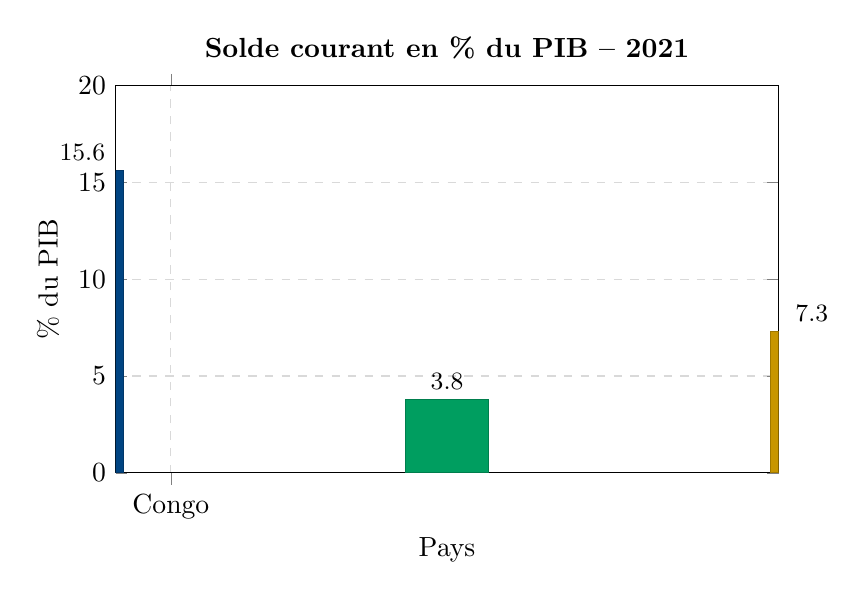
\begin{tikzpicture}
    \begin{axis}[
      ybar,
      width=10cm, height=6.5cm,
      bar width=30pt,
      xlabel={Pays},
      ylabel={\% du PIB},
      xtick=data,
      xticklabels={Congo, Gabon, Tchad},
      ymin=0, ymax=20,
      ytick={0,5,10,15,20},
      nodes near coords,
      nodes near coords align={vertical},
      every node near coord/.append style={font=\small\bfseries},
      title={\textbf{Solde courant en \% du PIB -- 2021}},
      title style={font=\normalsize\bfseries},
      grid=major, grid style={dashed,gray!30},
    ]
    \addplot[fill={congoblue}, draw=congoblue!80!black] coordinates {(1,15.6)};
    \addplot[fill={gabongreen}, draw=gabongreen!80!black] coordinates {(2,3.8)};
    \addplot[fill={tchadyellow}, draw=tchadyellow!80!black] coordinates {(3,7.3)};
    \end{axis}
  \end{tikzpicture}
  \caption{Solde du compte courant rapporté au PIB (2021)}
  \label{fig:solde_pib}
\end{figure}

Le Congo affiche le ratio le plus élevé (+15,6\,\% du PIB), reflétant sa concentration
extrême sur le pétrole. Un excédent courant aussi élevé est en général associé, dans la
littérature, à une sous-consommation nationale et à une forte captation de la valeur ajoutée
par les non-résidents \parencite{krugmanobstfeld2018}. Le Tchad (+7,3\,\%) se situe en
position intermédiaire, tandis que le Gabon (+3,8\,\%), bien qu'excédentaire, est le pays
dont la position courante est la plus fragile, en raison du poids disproportionné des
sorties de services.

\subsubsection{Décomposition du solde courant}

\begin{figure}[h!]
  \centering
  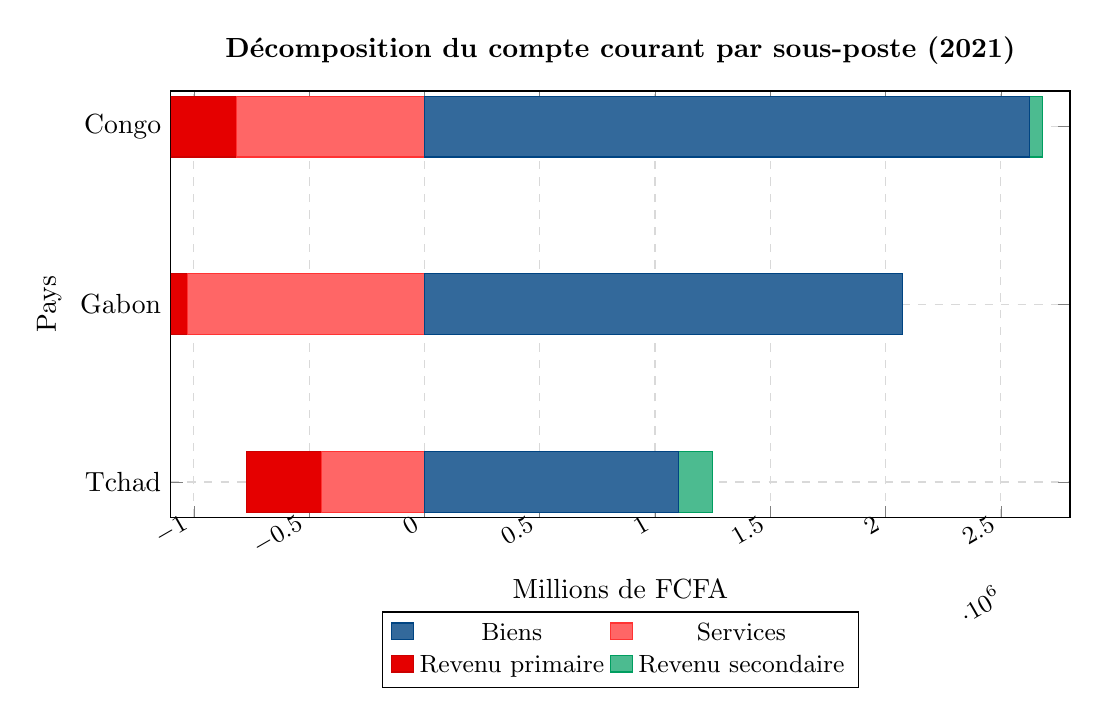
\begin{tikzpicture}
    \begin{axis}[
      xbar stacked,
      width=13cm, height=7cm,
      bar width=22pt,
      xlabel={Millions de FCFA},
      ylabel={Pays},
      ytick=data,
      yticklabels={Tchad, Gabon, Congo},
      xmin=-1100000, xmax=2800000,
      xtick={-1000000,-500000,0,500000,1000000,1500000,2000000,2500000},
      xticklabel style={font=\small, rotate=30, anchor=east},
      legend style={at={(0.5,-0.22)}, anchor=north, legend columns=2, font=\small},
      title={\textbf{Décomposition du compte courant par sous-poste (2021)}},
      title style={font=\normalsize\bfseries},
      grid=major, grid style={dashed,gray!30},
    ]
    % Biens
    \addplot[fill=congoblue!80, draw=congoblue] coordinates {
      (1101693,1) (2072410,2) (2624146,3)
    };
    % Services
    \addplot[fill=red!60, draw=red!80] coordinates {
      (-447358,1) (-1026580,2) (-813677,3)
    };
    % Revenu primaire
    \addplot[fill=red!90!black, draw=red!80!black] coordinates {
      (-325471,1) (-639322,2) (-915344,3)
    };
    % Revenu secondaire
    \addplot[fill=gabongreen!70, draw=gabongreen] coordinates {
      (147884,1) (-32878,2) (56398,3)
    };
    \legend{Biens, Services, Revenu primaire, Revenu secondaire}
    \end{axis}
  \end{tikzpicture}
  \caption{Décomposition du compte courant (2021)}
  \label{fig:decomp_courant}
\end{figure}

La figure \ref{fig:decomp_courant} illustre clairement le profil commun des trois économies
et leurs différences structurelles. Le Gabon se distingue par le déficit des services le
plus lourd en valeur absolue ($-$1\,026\,580 M FCFA), tandis que le Congo présente le déficit
du revenu primaire le plus profond ($-$915\,344 M FCFA). Le Tchad se démarque par un revenu
secondaire excédentaire (+147\,884 M FCFA), reflétant sa forte dépendance à l'aide
internationale, y compris les fonds des organisations humanitaires opérant sur son territoire.

\subsection{Diagnostic macroéconomique synthétique}

\begin{table}[h!]
  \centering
  \caption{Tableau de bord comparatif -- Congo, Gabon, Tchad (2021)}
  \label{tab:diagnostic}
  \begin{tabularx}{\linewidth}{X r r r}
    \toprule
    \textbf{Indicateur}              & \textbf{Congo} & \textbf{Gabon} & \textbf{Tchad} \\
    \midrule
    Solde courant (M FCFA)           & +951\,523 & +373\,630 & +476\,748 \\
    Solde courant / PIB              & +15,6\,\% &  +3,8\,\% &  +7,3\,\% \\
    Solde biens / PIB                & +43,1\,\% & +20,9\,\% & +16,9\,\% \\
    Taux de couverture biens         &  2,70     &   2,08    &  2,04     \\
    Taux d'absorption services       & 19,5\,\%  & 25,7\,\%  & 20,7\,\%  \\
    Taux de fuite revenu primaire    & 22,0\,\%  & 16,0\,\%  & 15,0\,\%  \\
    \textbf{Taux de rétention}       & \textbf{58,5\,\%} & \textbf{58,3\,\%} & \textbf{64,3\,\%} \\
    Capacité de financement (M FCFA) & +965\,295 & +351\,664 & +620\,351 \\
    Erreurs \& Omissions (M FCFA)   & +34\,478  & +310\,772 & $-$233\,149 \\
    Qualité statistique              & Bonne     & Faible    & Moyenne   \\
    \bottomrule
  \end{tabularx}

  \smallskip
  \footnotesize\textit{Source : Calculs de l'auteur à partir des fichiers BEAC 2021 et FMI WEO 2022.}
\end{table}

Le tableau \ref{tab:diagnostic} confirme que les trois économies partagent un profil
structurel commun caractéristique des économies de rente pétrolière au sens de
\textcite{sachswarner1995} : forte dépendance aux exportations d'une ressource non
renouvelable, faibles taux de rétention des revenus d'exportation, et vulnérabilité aiguë
aux chocs externes sur les prix des matières premières. En appliquant le cadre de
\textcite{cordenneary1982}, on identifie les symptômes classiques du syndrome hollandais :
atrophie du secteur des services exportables, captation de la valeur ajoutée extractive par
des acteurs non-résidents, et absence de diversification productive.

%% ══════════════════════════════════════════════════════════════════════════
\section{Conclusion}
%% ══════════════════════════════════════════════════════════════════════════

Cette analyse comparative de la balance des paiements du Congo, du Gabon et du Tchad en
2021 conduit à trois conclusions principales.

\textbf{Premièrement}, les trois pays sont excédentaires en courant en 2021 grâce au rebond
des cours pétroliers, mais cet excédent est entièrement conjoncturel et repose sur une
ressource épuisable. La structure interne des comptes révèle des déficits structurels
profonds des services et du revenu primaire, dont le niveau ne dépend pas du prix du pétrole.

\textbf{Deuxièmement}, les termes d'échange, favorables en 2021 grâce à la hausse des cours,
masquent une rétention nationale de la valeur exportée inférieure à 65\,\% pour les trois
pays. Les 35 à 42\,\% restants fuient vers l'étranger via les paiements de services techniques
et les revenus des investissements directs. Ce mécanisme, conforme aux prédictions du modèle
de \textcite{cordenneary1982}, constitue un frein structurel au développement.

\textbf{Troisièmement}, des différences significatives existent entre les trois pays : le
Congo est le plus concentré sur le pétrole et le plus exposé au déficit de revenu primaire ;
le Gabon présente le déficit de services le plus élevé et les données statistiques les moins
fiables ; le Tchad bénéficie d'une aide internationale massive qui structure positivement
son compte courant et de capital, mais crée une double dépendance fragile.

Ces résultats appellent des politiques économiques de diversification structurelle urgentes
dans les trois pays, notamment le développement d'industries de transformation locale, le
renforcement du contenu local dans les contrats pétroliers, et la constitution de fonds
souverains permettant de lisser les chocs de revenus pétroliers, sur le modèle des
recommandations de \textcite{imfcemac2021}.

%% ══════════════════════════════════════════════════════════════════════════
\printbibliography[title={Références bibliographiques}]
%% ══════════════════════════════════════════════════════════════════════════

\end{document}
